\subsection{Section 8.3}

\begin{tcolorbox}[
        title={Problem 10 (a)},
        valign=center,
        nobeforeafter,
        colframe=gray!95!black
    ]
    Show that
    \begin{align}
        \vb{F} &= -\frac{\vb{r}}{|\vb{r}|^3}
    \end{align}
    is the gradient of the function \(f(x, y, z) = \frac{1}{r}\).
\end{tcolorbox}

\begin{proof}
\textit{(Cartesian coordinates)}

Recall that the gradient operator in Cartesian coordinates is given by:
\begin{align}
    \nabla &= \left(\frac{\partial}{\partial x}, \frac{\partial}{\partial y}, \frac{\partial}{\partial z}\right)
\end{align}

Then:
\begin{align*}
    \nabla f &= \nabla \left(\frac{1}{r}\right) \\
    &= \nabla \left(\frac{1}{\sqrt{x^2 + y^2 + z^2}}\right) \\
    &= \left(-\frac{2x}{2(x^2 + y^2 + z^2)^{\frac{3}{2}}}, -\frac{2y}{2(x^2 + y^2 + z^2)^{\frac{3}{2}}}, -\frac{2z}{2(x^2 + y^2 + z^2)^{\frac{3}{2}}}\right) \\
    &= \left(-\frac{x}{(x^2 + y^2 + z^2)^{\frac{3}{2}}}, -\frac{y}{(x^2 + y^2 + z^2)^{\frac{3}{2}}}, -\frac{z}{(x^2 + y^2 + z^2)^{\frac{3}{2}}}\right) \\
    &= \left(-\frac{x}{r^3}, -\frac{y}{r^3}, -\frac{z}{r^3}\right) \\
    &= -\frac{\left(x, y, z\right)}{r^{3}} \\
    &= -\frac{\vb{r}}{r^{3}} \\
    &= -\frac{\vb{r}}{|\vb{r}|^{3}} \\
    &=\vb{F}
\end{align*}

Therefore, we have proven that \(\nabla f = \vb{F}\).
\end{proof}

\begin{tcolorbox}[
        title={Problem 10 (b)},
        valign=center,
        nobeforeafter,
        colframe=gray!95!black
    ]
    What is the work done by the force \(\vb{F} = -\frac{\vb{r}}{|\vb{r}|^3}\) in moving a particle from a point \(\vb{r}_0 \in \mathbb{R}^3\) to \(\infty\), where \(\vb{r}(x, y, z) = (x, y, z)\)?
\end{tcolorbox}

\begin{solution}
    Let \(\vb{c}\) be a \(C^1\) curve and let \(f: \mathbb{R}^3 \rightarrow \mathbb{R}\) be a \(C^1\) function. 
    
    Recall by chain rule that:
    \begin{align}
        \frac{d}{dt} f(\vb{c}(t)) &= \nabla f(\vb{c}(t)) \cdot \vb{c}'(t)
    \end{align}
    
    \newpage
    
    Now let \(\vb{c}: [0, 1] \rightarrow \mathbb{R}^3 \backslash (0,0,0)\) be a \(C^1\) curve where \(\vb{c}(0) = \vb{r}_0\) and \(\vb{c}(1) = \vb{r}_1\). Note that we omit the point \((0, 0, 0)\) from our curve since \(\vb{F}(x, y, z)\) is not defined at \((0, 0, 0)\).
    
    The work done by the force \(\vb{F}\) along \(\vb{c}(t)\) is given by:
    \begin{align*}
        W(\vb{r}_0, \vb{r}_1) &= \int_c \vb{F} \cdot d \vb{s} \\
        &= \int_0^1 \vb{F}(\vb{c}(t)) \cdot \vb{c}'(t) \ dt \\
        &= \int_0^1 \nabla f(\vb{c}(t)) \cdot \vb{c}'(t) \ dt \\
        &= \int_0^1 \frac{d}{dt} f(\vb{c}(t)) \ dt \\
        &= f(\vb{c}(1)) - f(\vb{c}(0)) \\
        &= f(\vb{r}_1) - f(\vb{r}_0) \\
        &= \frac{1}{|\vb{r}_1|} - \frac{1}{|\vb{r}_0|} \\
        &= \frac{1}{r_1} - \frac{1}{r_0}
    \end{align*}
    
    Since we want to move the particle from \(\vb{r}_0\) to \(\infty\), let \(r_1 \rightarrow \infty\).
    
    Then:
    \begin{align*}
        W(\vb{r}_0, \infty) &= \lim_{r_1 \rightarrow \infty} \frac{1}{r_1} - \frac{1}{r_0} \\
        &= 0 - \frac{1}{r_0} \\
        &= - \frac{1}{r_0} 
    \end{align*}
    
    Note that this work is negative, which can be understood physically by the fact that \(\vb{F}\) is an attractive force, and so we are working against it to go to \(\infty\).
\end{solution}

\begin{tcolorbox}[
        title={Problem 20},
        valign=center,
        nobeforeafter,
        colframe=gray!95!black
    ]
    Prove that if \(\vb{F}\) is a divergence-free \(C^1\) vector field on all of \(\mathbb{R}^3\), then there exists a \(C^1\) vector field \(\vb{G}\) with \(\vb{F} = \nabla \times \vb{G}\). \\
    
    Hint: Define \(\vb{G} = (G_1, G_2, G_3)\) by:
    \begin{align}
        G_1(x, y, z) &= \int_0^z F_2(x, y, t) \ dt - \int_0^y F_3(x, t, 0) \ dt \\
        G_2(x, y, z) &= -\int_0^z F_1(x, y, t) \ dt \\
        G_3(x, y, z) &= 0
    \end{align}
\end{tcolorbox}

\begin{proof}
    Suppose that \(\nabla \cdot \vb{F} = 0\).
    
    We first write out the curl of \(\vb{G}\) explicitly:
    \begin{align}
        \nabla \times \vb{G} &= \left(\frac{\partial G_3}{\partial y} - \frac{\partial G_2}{\partial z}\right) \vb{i} + \left(\frac{\partial G_1}{\partial z} - \frac{\partial G_3}{\partial x}\right) \vb{j} + \left(\frac{\partial G_2}{\partial x} - \frac{\partial G_1}{\partial y}\right) \vb{k} 
    \end{align}
    
    We now compute the necessary partial derivatives of \(G_1\), \(G_2\), and \(G_3\) by frequently applying the Fundamental Theorem of Calculus:
    \begin{align*}
        \frac{\partial G_1}{\partial y} &= \frac{\partial}{\partial y} \left(\int_0^z F_2(x, y, t) \ dt - \int_0^y F_3(x, t, 0) \ dt\right) \\
        &= \frac{\partial}{\partial y} \int_0^z F_2(x, y, t) \ dt - \frac{\partial}{\partial y} \int_0^y F_3(x, t, 0) \ dt \\
        &= \int_0^z \frac{\partial}{\partial y} F_2(x, y, t) \ dt - F_3(x, y, 0) \\
        \\
        \frac{\partial G_1}{\partial z} &= \frac{\partial}{\partial z} \left(\int_0^z F_2(x, y, t) \ dt - \int_0^y F_3(x, t, 0) \ dt\right) \\
        &= \frac{\partial}{\partial z} \int_0^z F_2(x, y, t) \ dt - \frac{\partial}{\partial z} \int_0^y F_3(x, t, 0) \ dt \\
        &= F_2(x, y, z) - \int_0^y \frac{\partial}{\partial z} F_3(x, t, 0) \ dt \\
        &= F_2(x, y, z) - 0 \\
        &= F_2(x, y, z) \\
        \\
        \frac{\partial G_2}{\partial x} &= -\frac{\partial}{\partial x} \int_0^z F_1(x, y, t) \ dt \\
        &= - \int_0^z \frac{\partial}{\partial x} F_1(x, y, t) \ dt \\
        \\
        \frac{\partial G_2}{\partial z} &= -\frac{\partial}{\partial z} \int_0^z F_1(x, y, t) \ dt \\
        &= - F_1(x, y, z)
    \end{align*}
    
    Then, recalling that \(G_3 = 0\):
    \begin{align*}
        \nabla \times \vb{G} &= \left(\frac{\partial G_3}{\partial y} - \frac{\partial G_2}{\partial z}\right) \vb{i} + \left(\frac{\partial G_1}{\partial z} - \frac{\partial G_3}{\partial x}\right) \vb{j} + \left(\frac{\partial G_2}{\partial x} - \frac{\partial G_1}{\partial y}\right) \vb{k} \\
        &= - \frac{\partial G_2}{\partial z} \vb{i} + \frac{\partial G_1}{\partial z}\vb{j} + \left(\frac{\partial G_2}{\partial x} - \frac{\partial G_1}{\partial y}\right) \vb{k} \\
        &= - (- F_1(x, y, z)) \vb{i} + F_2(x, y, z) \vb{j} + \left(- \int_0^z \frac{\partial}{\partial x} F_1(x, y, t) \ dt - \int_0^z \frac{\partial}{\partial y} F_2(x, y, t) \ dt + F_3(x, y, 0)\right) \vb{k} \\
        &= F_1(x, y, z) \vb{i} + F_2(x, y, z) \vb{j} - \left(\int_0^z \frac{\partial}{\partial x} F_1(x, y, t) \ dt + \int_0^z \frac{\partial}{\partial y} F_2(x, y, t) \ dt - F_3(x, y, 0)\right) \vb{k}
    \end{align*}
    
    Observe that, by the Fundamental Theorem of Calculus:
    \begin{align*}
        \int_0^z \frac{\partial }{\partial t} F_3(x, y, t) \ dt &= F_3(x, y, z) - F_3(x, y, 0) \\
        \int_0^z \frac{\partial }{\partial t} F_3(x, y, t) \ dt - F_3(x, y, z) &= - F_3(x, y, 0)
    \end{align*}
    
    Then:
    \begin{align*}
        \nabla \times \vb{G} &= F_1(x, y, z) \vb{i} + F_2(x, y, z) \vb{j} - \left(\int_0^z \frac{\partial}{\partial x} F_1(x, y, t) \ dt + \int_0^z \frac{\partial}{\partial y} F_2(x, y, t) \ dt - F_3(x, y, 0)\right) \vb{k} \\
        &= F_1(x, y, z) \vb{i} + F_2(x, y, z) \vb{j} \\
        &\quad - \left(\int_0^z \frac{\partial}{\partial x} F_1(x, y, t) \ dt + \int_0^z \frac{\partial}{\partial y} F_2(x, y, t) \ dt + \int_0^z \frac{\partial }{\partial t} F_3(x, y, t) \ dt - F_3(x, y, z)\right) \vb{k} \\
        &= F_1(x, y, z) \vb{i} + F_2(x, y, z) \vb{j} \\
        &\quad - \left(\int_0^z \frac{\partial}{\partial x} F_1(x, y, t) + \frac{\partial}{\partial y} F_2(x, y, t) + \frac{\partial }{\partial t} F_3(x, y, t) \ dt - F_3(x, y, z)\right) \vb{k} \\
        &= F_1(x, y, z) \vb{i} + F_2(x, y, z) \vb{j} - \left(\int_0^z \nabla \cdot \vb{F}(x, y, t) \ dt - F_3(x, y, z)\right) \vb{k} \\
        &= F_1(x, y, z) \vb{i} + F_2(x, y, z) \vb{j} - \left(\int_0^z 0 \ dt - F_3(x, y, z)\right) \vb{k} \\
        &= F_1(x, y, z) \vb{i} + F_2(x, y, z) \vb{j} - \left(0 - F_3(x, y, z)\right) \vb{k} \\
        &= F_1(x, y, z) \vb{i} + F_2(x, y, z) \vb{j} + F_3(x, y, z) \vb{k} \\
        &= \vb{F}
    \end{align*}
    where we used the fact that \(\nabla \cdot \vb{F} = 0\) on all of \(\mathbb{R}^3\). 
\end{proof}

\subsection{Section 8.4}

\begin{tcolorbox}[
        title={Problem 14},
        valign=center,
        nobeforeafter,
        colframe=gray!95!black
    ]
    Let \(W\) be the three-dimensional solid enclosed by the surfaces \(x = y^2\), \(x = 9\), \(z = 0\), and \(x = z\). Let \(S\) be the boundary of \(W\). \\
    
    Use Gauss’ theorem to find the flux of \(\vb{F}(x, y, z) = (3x - 5y)\vb{i} + (4z - 2y)\vb{j} + (8yz)\vb{k}\) across \(S\).
\end{tcolorbox}

\begin{solution}
    Recall Gauss' Divergence Theorem:
    \begin{align}
        \iint_{\partial W} \vb{F} \cdot d\vb{S} &= \iiint_W \nabla \cdot \vb{F} \ dV
    \end{align}
    
    Since \(S = \partial W\), the surface integral is given by:
    \begin{align*}
        \iint_{S} \vb{F} \cdot d\vb{S} &= \iiint_W \nabla \cdot \vb{F} \ dV \\
        &= \iiint_W \nabla \cdot (3x - 5y, 4z - 2y, 8yz) \ dV \\
        &= \iiint_W 3 - 2 + 8y \ dV \\
        &= \iiint_W 1 + 8y \ dV
    \end{align*}
    
    \newpage 
    
    \begin{figure}[h!]
        \centering
        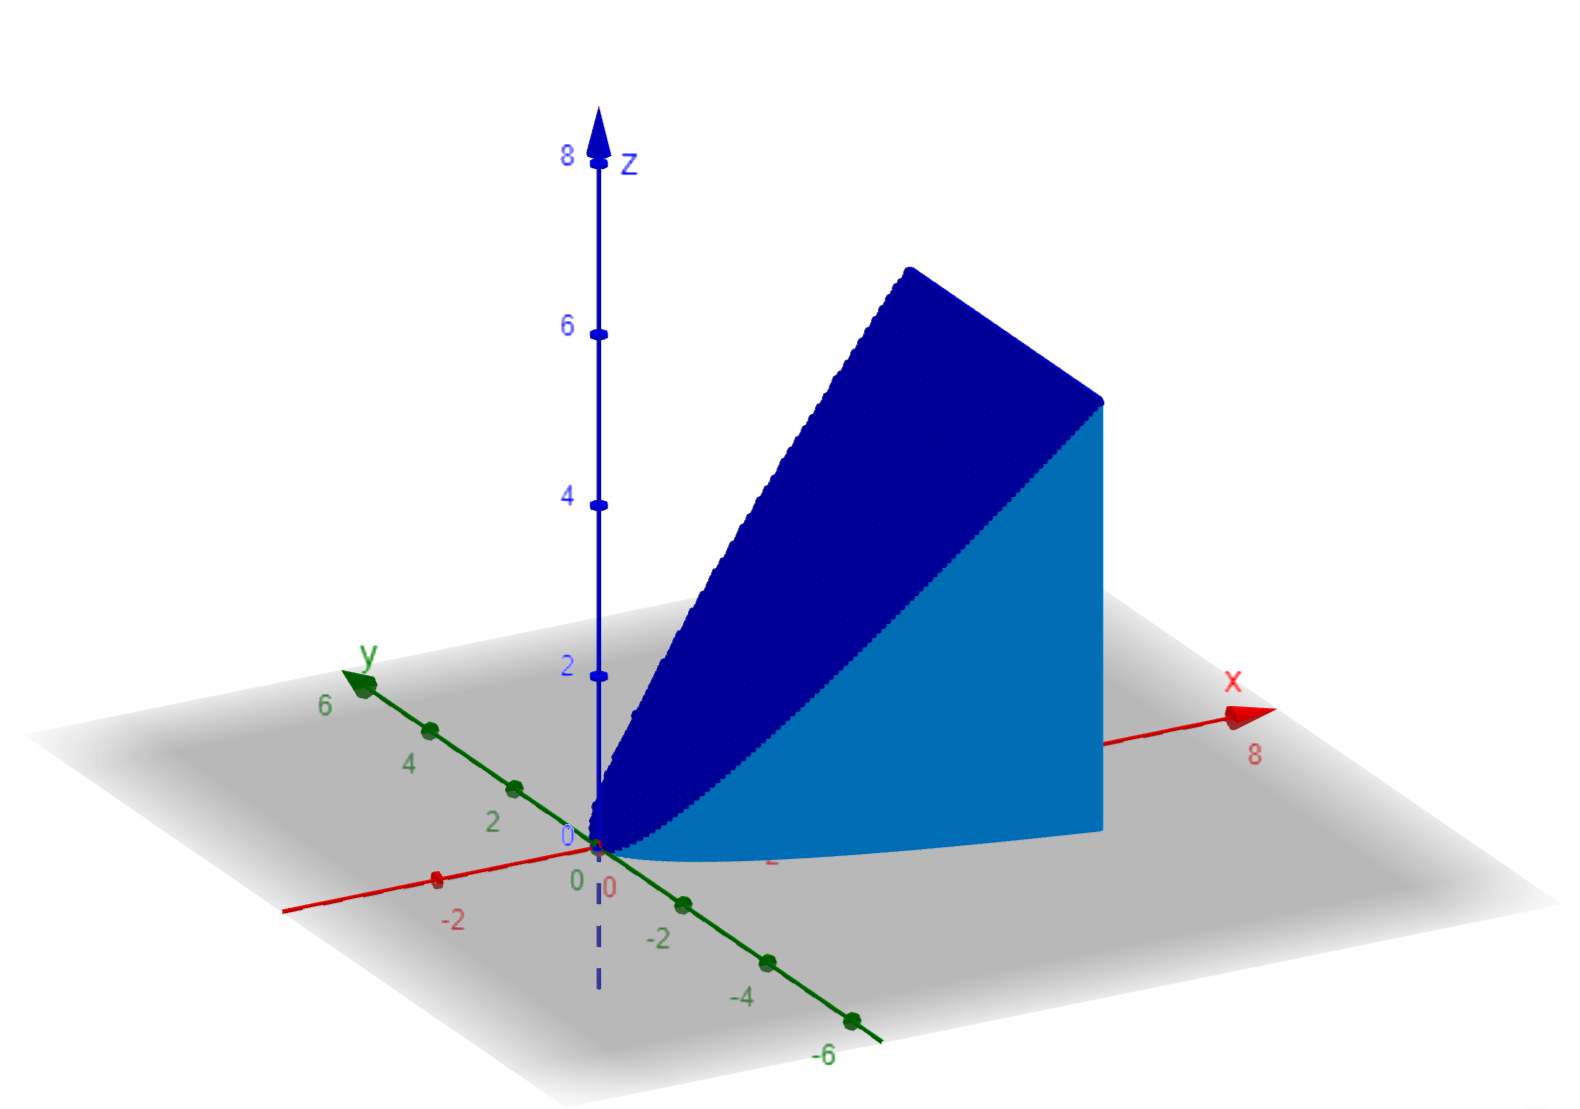
\includegraphics[width=0.7\textwidth]{Pictures/Tutorial 10-1.png} \\
        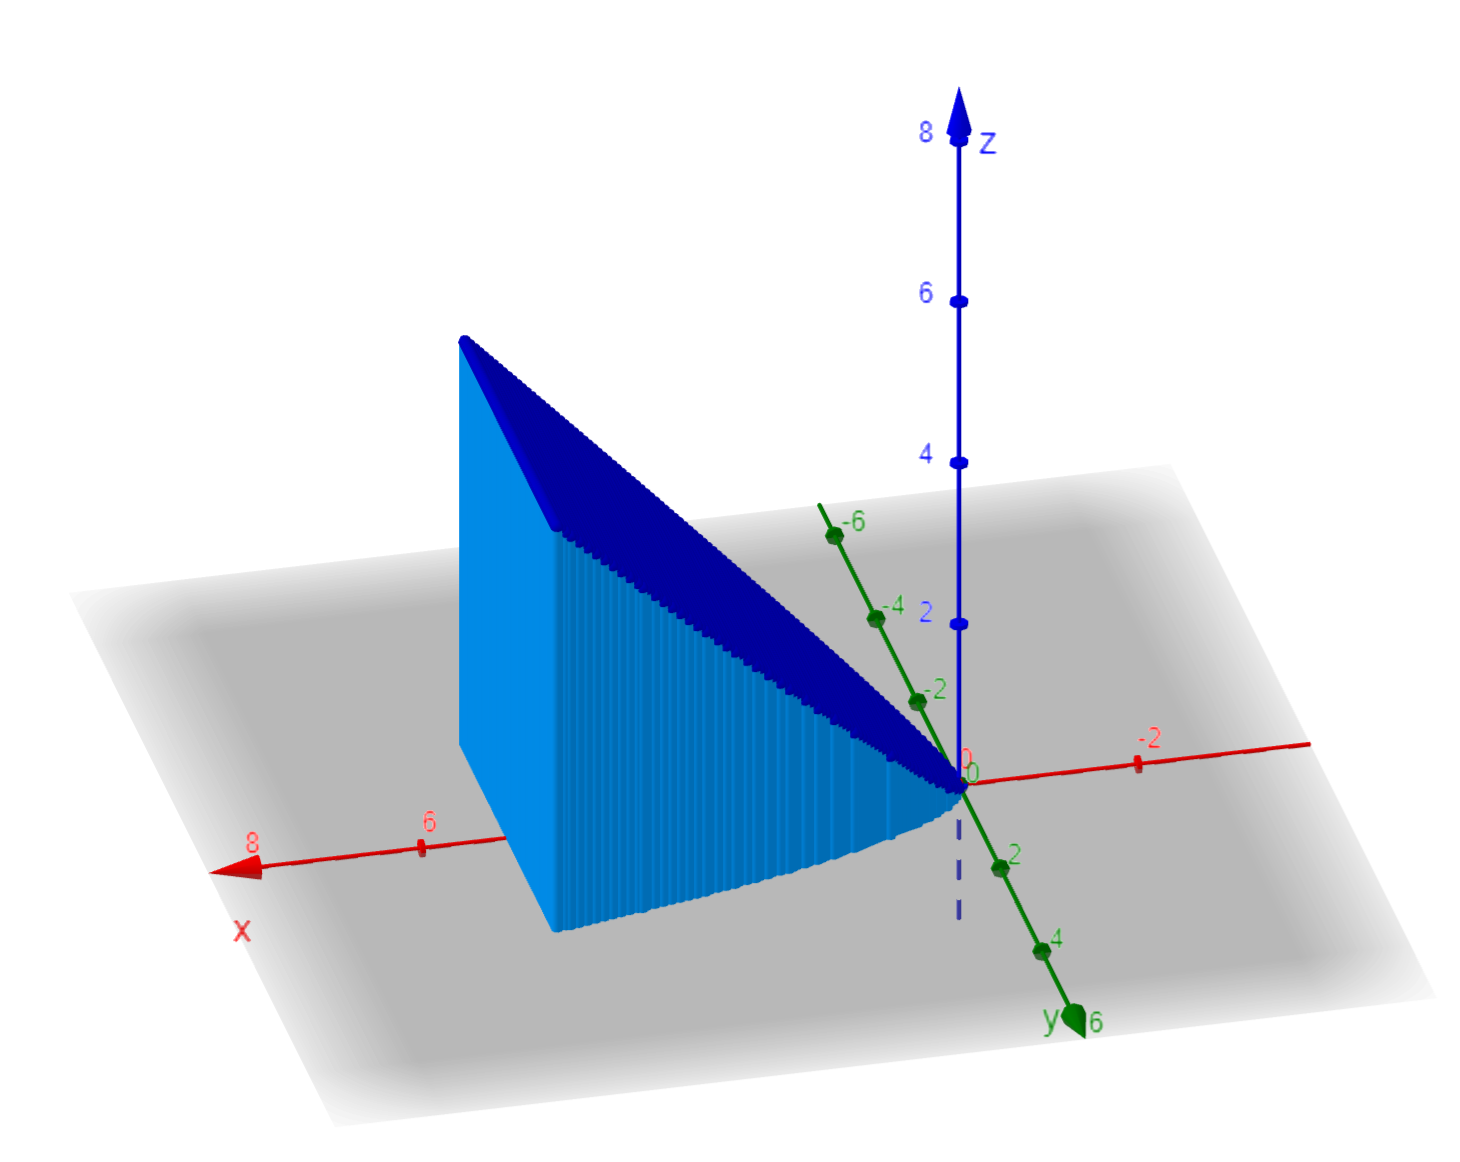
\includegraphics[width=0.7\textwidth]{Pictures/Tutorial 10-2.png}
        \caption{Visualizing the region \(W\) in 3D.}
    \end{figure}
    
    By observation:
    
    The upper bound of \(z\) is given by \(z = x\). 
    The lower bound of \(z\) is given by \(z = 0\). 
    
    The upper bound of \(x\) is found to be \(x = 9\). 
    The upper bound of \(x\) is found to be \(x = y^2\).
    
    The upper bound of \(y\) is found to be \(y = 3\).
    The upper bound of \(y\) is found to be \(y = -3\).
    
    The bounds of our integral should therefore be:
    \begin{align}
        0 \leq & \ z \leq x & y^2 \leq & \ x \leq 9 & -3 \leq & \ y \leq 3
    \end{align}
    
    Other bounds (with different integration orders) may also be correct.
    
    Then:
    \begin{align*}
        \iint_{S} \vb{F} \cdot d\vb{S} &= \iiint_W 1 + 8y \ dV \\
        &= \int_{-3}^3 \int_{y^2}^9 \int_0^x 1 + 8y \ dzdxdy \\
        &= \int_{-3}^3 \int_{y^2}^9 (1 + 8y) z \Big|_{z = 0}^{z = x} \ dxdy \\
        &= \int_{-3}^3 \int_{y^2}^9 (1 + 8y) x \ dxdy \\
        &= \int_{-3}^3 (1 + 8y) \frac{x^2}{2} \Biggr|_{x = y^2}^{x = 9} \ dy \\
        &= \int_{-3}^3 (1 + 8y) \left(\frac{9^2}{2} - \frac{y^4}{2}\right) \ dy \\
        &= \int_{-3}^3 \left(\frac{81}{2} - \frac{y^4}{2}\right) + 8y\left(\frac{81}{2} - \frac{y^4}{2}\right) \ dy \\
        &= \int_{-3}^3 \frac{81}{2} - \frac{y^4}{2} + 324y - 4y^5 \ dy \\
        &= \left(\frac{81y}{2} - \frac{y^5}{10} + 162y^2 - \frac{2y^6}{3}\right) \Biggr|_{-3}^3 \\
        &= 243 - \frac{243}{5}
    \end{align*}
\end{solution}

\begin{tcolorbox}[
        title={Problem 16},
        valign=center,
        nobeforeafter,
        colframe=gray!95!black
    ]
    Evaluate the surface integral:
    \begin{align}
        \iint_{S} \vb{F} \cdot \vb{n} \ dA
    \end{align}
    where \(\vb{F}(x, y, z) = \vb{i} + \vb{j} + z(x^2 + y^2)^2\vb{k}\) and \(S\) is the surface of the cylinder \(x^2 + y^2 \leq 1\) with \(0 \leq z \leq 1\).
\end{tcolorbox}

\begin{solution}
    Rather than computing the flux of \(\vb{F}\) through the three sides of the cylinder, we may compute the volume integral of \(\nabla \cdot \vb{F}\) over the region \(W\) bounded by the cylinder using the Divergence Theorem.
    
    Recall the Divergence Theorem:
    \begin{align}
        \iint_S \vb{F} \cdot d\vb{S} &= \iiint_W \nabla \cdot \vb{F} \ dV
    \end{align}
    
    Then the surface integral is given by:
    \begin{align*}
        \iint_{S} \vb{F} \cdot \vb{n} \ dA &= \iiint_W \nabla \cdot \vb{F} \ dV \\
        &= \iiint_W \nabla \cdot (1, 1, z(x^2 + y^2)^2) \ dV \\
        &= \iiint_W 0 + 0 + (x^2 + y^2)^2 \ dV \\
        &= \iiint_W (x^2 + y^2)^2 \ dV 
    \end{align*}
    
    Recall cylindrical coordinates:
    \begin{align}
        x^2 + y^2 &= r^2 & dV &= r \ dr d\theta dz
    \end{align}
    
    Then:
    \begin{align*}
        \iint_{S} \vb{F} \cdot \vb{n} \ dA &= \iiint_W (x^2 + y^2)^2 \ dV \\
        &= \int_0^1 \int_0^{2\pi} \int_0^1 (r^2)^2 r \ dr d\theta dz \\
        &= \int_0^1 r^5 \ dr \int_0^{2\pi} d\theta \int_0^1 dz \\
        &= \frac{r^6}{6} \Biggr|_0^1 \int_0^{2\pi} d\theta \int_0^1 dz \\
        &= \frac{1}{6} (2\pi) (1) \\
        &= \frac{\pi}{3}
    \end{align*}
\end{solution}
